\chapter{Popis problematiky}
V mnoha oblastech lidské činnosti existují problémy, které je možné popsat s využitím omezujících podmínek. Ať už je to generování školního rozvrhu (kde jednou z omezujících podmínek může být například volný čas jednotlivých vyučujících), či vyhýbání se překážkám u samořídících automobilů, obecně jde vždy o nějaký problém, pro který je potřeba najít optimální řešení při splnění daných omezení. Těmto problémům se říká \emph{constraint satisfaction problems} (CSP, česky \emph{problémy splnitelnosti omezujících podmínek}).






\section{Constraint programming}
\emph{Constraint programming} (či \emph{programování s omezujícími podmínkami}) je jedním z odvětví umělé inteligence pro řešení optimalizačních úloh (konkrétně CSP úloh). Asociace ACM v \cite{Wegner1996} označila toto téma jako jedno z klíčových oblastí pro budoucí výzkum, neboť se problémy s omezujícími podmínkami přirozeně vyskytují v každodenním životě. Předností constraint programming je navíc to, že uživatel popíše problém k vyřešení pouze deklarativně - nedá tedy počítači žádný postup k řešení, jen zadá aktuální stav problému a specializovaný program (řešič) najde řešení (pokud existuje).

Typickým příkladem problému s omezujícími podmínkami jsou různé hry, například sudoku. Jak ukazuje definice \ref{def:csp}, CSP se skládá z proměnných, domén a omezujících podmínek. V sudoku jsou proměnnými volná políčka na hracím poli, z nichž každá má svoji \emph{doménu} (množinu hodnot, kterých může teoreticky nabývat, v tomto případě čísla 1 a 9). Omezujícími podmínkami jsou samotná pravidla hry - požadavek na unikátnost číslice v řádku, sloupci, resp. ve~čtverci. Pojmy \emph{doména} a \emph{omezující podmínka} přesněji vysvětlují následující podkapitoly.

\begin{definition}
\label{def:csp}
\emph{CSP} (\emph{problém splnitelnosti omezujících podmínek}) je trojice $(V, D, C)$, kde
\begin{itemize}
  \item $V$ je uspořádaná posloupnost proměnných,
  \item $D$ je uspořádaná posloupnost domén náležejících k proměnným,
  \item $C$ je množina omezujících podmínek.
\end{itemize}
\end{definition}

Známý SAT problém\footnote{Boolean satisfiability problem} je také příkladem problému s omezujícími podmínkami.

\subsection{Doména}
\begin{definition}
\label{def:domain}
\emph{Doména} (nebo také \emph{definiční obor}) proměnné je množina všech hodnot, kterých může proměnná nabývat.
\end{definition}

Doménou, jak ukazuje definice \ref{def:domain}, může být jakákoliv množina. Domény mohou být diskrétní (podmnožina přirozených čísel, ${red, green, blue}$ při obarvování grafu, ${true, false}$ u SAT problém, apod.) či spojité (interval reálných čísel)


\subsection{Omezující podmínka}
\begin{definition}
\label{def:constraint}
\emph{Omezující podmínka} $c$ na konečné posloupnosti proměnných\\$(x_1, \dots, x_n)$ s doménami $(\boldsymbol{D_1}, \dots, \boldsymbol{D_n})$, $n \in \boldsymbol{N}$, je podmnožina kartézského součinu $\boldsymbol{D_1} \times \dots \times \boldsymbol{D_n}$.
\end{definition}

Omezující podmínka dle definice \ref{def:constraint} je tedy relace mezi proměnnými a lze ji zapsat jako $c(x_1, \dots, x_n)$. Vzhledem k tomu, že se jedná o relaci, lze omezující podmínky rozdělit podle arity na relace na unární ($x \leq 1$), binární ($x = y$) a více-ární ($x + y > z $).

V praktické části této práce budou omezující podmínky reprezentovány rovnicemi (jednoduchá rovnice $x = 0, x \in \boldsymbol{N}$ zjevně omezuje možné hodnoty proměnné $x$, jedná se tedy o omezující podmínku).

Omezující podmínka je \emph{redundantní} (nadbytečná), nemá-li její odebrání z CSP vliv na řešení problému (v problému \\ $P = (V, D, C)$, kde $C = {c_1: x > y, c_2: x > y, c_3: y < x}$ jsou libovolné dvě podmínky redundantní).

(TODO: později třeba zmínit, že program neprovádí detekci redundantních podmínek a že to je prostor pro zlepšení...)

Pro práci je důležité ještě jedno dělení omezujících podmínek, a to na \emph{primitivní} a \emph{komplexní} podmínky (více viz \cite{kue12}). Omezující podmínka reprezentovaná rovnicí v primitivním tvaru obsahuje maximálně dvě aritmetické operace (maximální arita podmínky je tedy rovna třem). Toto rozdělení je důležité, protože algoritmus využitý v praktické části umí pracovat pouze s primitivními podmínkami a program je očekává na vstupu. Je tedy před spuštěním programu provést manuální rozklad podmínek a označit, které z proměnných se vyskytovaly v původních podmínkách. Takovým proměnným se říká \emph{dominantní}, ostatní jsou \emph{nedominantní}, nebo také \emph{pomocné} proměnné.

Rozdíl mezi ekvivalentními jednoduchými a komplexními podmínkami ukazují příklady č. \ref{eq:complexConstraint} a \ref{eq:primitiveConstraint}. V tomto příkladu jsou dominantními proměnné $x$, $y$ a $z$.

\begin{equation} \label{eq:complexConstraint}
x + 2y + z = 1
\end{equation}

\begin{equation} \label{eq:primitiveConstraint}
v_1 = 2y \quad \wedge \quad v_2 = z - 1 \quad \wedge \quad v_3 = x + v_1 \quad \wedge \quad v_3 + v_2 = 0
\end{equation}







\section{Numerical constraint satisfaction problem}

Tato práce se zabývá řešením \emph{numerických CSP} (\emph{NCSP}, \emph{numerical CSP}), což je podmnožina CSP problémů, jejichž domény jsou spojité (a tedy jsou to intervaly) a které se dají reprezentovat soustavami rovnic či nerovnic. Rovnice nebo nerovnice vlastně kladou na proměnné nějaká omezení a zmenšují tak množiny hodnot, kterých mohou nabývat.

Domény proměnných v NCSP problémech jsou reálné intervaly, a cílem je co nejvíce tyto intervaly zúžit (zúžení domény podle omezující podmínky se říká \emph{propagace omezující podmínky}), aby ale stále byly všechny omezující podmínky splněny, viz jednoduchý příklad \ref{eq:simpleConstraint}.

\begin{equation} \label{eq:simpleConstraint}
x^2 = 1\qquad x \in \boldsymbol{R}
\end{equation}

Nechť rovnice \ref{eq:simpleConstraint} představuje omezující podmínku a pro doménu $D_x$ proměnné $x$ platí $D_x = (-5;5)$. Všechna řešení této rovnice určitě leží v intervalu $D_x$, ale také například v $\langle -1;2)$, nikoliv však v $(0;2)$ (tento interval obsahuje jen jedno ze dvou řešení). Metody řešení numerických CSP dokáží problém vyřešit nalezením minimálního intervalu obsahujícího všechna řešení, tj. $D_x' = \langle -1;1\rangle$. Nalezený interval vlastně tvoří jakési ohraničení všech možných řešení, anglicky se toto ohraničení nazývá \emph{box}. V praxi je pak třeba řešit soustavy těchto podmínek a nalezená ohraničení (boxy) jsou tvořena kartézským součinem intervalů.

Výhodou těchto problému je fakt, že se dají (alespoň do počtu třech dominantních proměnných) snadno vizualizovat jako graf. Domény proměnných představují jednotlivé osy, omezující podmínky jsou funkce a boxy obalující řešení jsou skutečnými 2D či 3D \uv{krabicemi} okolo řešení.

Nebude-li řečeno jinak, bude se zbývající text právě věnovat především problematice numerických CSP.





\section{Řešení a splnitelnosti CSP}
Přiřazení konkrétní hodnoty z domény proměnné se nazývá \emph{ohodnocení} (\emph{label}). Přiřazuje-li ohodnocení hodnotu všem proměnným problému, jedná se o \emph{úplné ohodnocení} (\emph{compound label}). Tyto pojmy stačí k definici řešení a splnitelnosti problému s omezujícími podmínkami (definice \ref{def:solution}, resp. \ref{def:satisfiability}).

\begin{definition}
\label{def:solution}
\emph{Řešení} (\emph{solution}) CSP je takové úplné ohodnocení, pro které platí všechny omezující podmínky.
\end{definition}

\begin{definition}
\label{def:satisfiability}
CSP problém je \emph{splnitelný} (\emph{satisfiable}), existuje-li pro něj řešení.
\end{definition}

Podle charakteru problému někdy stačí nalézt jen jedno řešení, jindy je třeba nalézt všechna řešení, jindy je nutné najít optimální řešení.

Jak ale vůbec řešení problému probíhá? Nejprve je nutné zavést pojmy \emph{ekvivalence problémů} a \emph{redukce problému}. Dva CSP problémy jsou ekvivalentní, jsou-li nadefinované nad~stejnou posloupností proměnných a stejnou množinou omezujících podmínek a mají stejné množiny řešení. Například problémy

\begin{align*}
P_1 = ((x, y), (\{-1,0,1,2,3\}, \{1,2,3\}), \{x - y = 0\}) \\
P_2 = ((x, y), (\{1,2,3\}, \{1,2,3\}), \{x - y = 0\})
\end{align*}

jsou ekvivalentní a splnitelné. Na stejném příkladu lze demonstrovat i redukci problému. Redukce problému je transformace na ekvivalentní a jednodušší CSP. Problém $P_2$ tak mohl vzniknout z~problému $P_1$ redukcí domény proměnné $x$, přičemž byly z domény dané proměnné odebrány tzv. \emph{nekonzistentní} hodnoty (hodnoty, pro které neexistuje řešení). Jak redukce může probíhat podrobně vysvětluje kapitola \ref{ch:searchReduction}, v tuto chvíli ji stačí považovat za černou skříňku, která na vstupu přijme CSP a vrátí ekvivalentní zredukovaný problém.

Obecný postup pro řešení CSP, který je popsán algoritmem~\ref{alg:GeneralSolutionAlg} (převzatý z~\cite[s.~22]{Vu2005}) využívá k~nalezení řešení právě redukování problému.

\begin{algorithm}
\caption{Algoritmus Solve}
\label{alg:GeneralSolutionAlg}
\begin{algorithmic}[1]
\Require Problém $P$ k vyřešení
\Ensure Řešení problému $P$
\Procedure{Solve}{$P$}
\State $continue \gets true$
\While{continue and not Happy}
\State Zredukuj problém $P$
\If{not Happy}
\If{atomic}
\State $continue \gets false$
\Else
\State \verb|Split| - rozděl problém a opakuj pro jednotlivé části
\EndIf
\EndIf
\EndWhile
\EndProcedure
\end{algorithmic}
\end{algorithm}

Algoritmus \verb|Solve| má tři důležité části - volání \verb|Happy| funkce, ověření \emph{atomicity} a rozdělení zredukovaného problému (\emph{splitting}). Spuštění algoritmu navíc často předchází předzpracování zadaného problému, jako například detekce a odstranění redundantních podmínek, nebo rozklad komplexních podmínek na primitivní.

\begin{itemize}
    \item Funkce \verb|Happy| ověřuje, jestli je program \uv{spokojený} s aktuálním výsledkem a jestli může skončit. To může znamenat například to, jestli byl nalezen dostatečný počet řešení, nebo jestli bylo dokázáno, že žádné řešení neexistuje, apod.
    \item Ověření atomicity je kontrola, zda je zredukovaný problém již dostatečně malý, aby byl přijat jako řešení. Pro určení velikosti problému lze využít několik metrik, v případě NCSP se nejčastěji používá měření velikosti domén dominantních proměnných a to buďto absolutní, nebo relativní vzhledem k původní velikosti (například požadavek na zmenšení domény na tisícinu původní velikosti).
    \item Nebyl-li problém dostatečně zmenšen, dojde k jeho rozdělení na více částí (resp. na několik menších CSP). To v praxi nejčastěji znamená, že dojde k rozdělení domén podle pravidla, kterých lze vymyslet poměrně velké množství. U CSP s diskrétními doménami je jedno z možných rozdělení takové, kdy se z domény nějaké proměnné vyjme jedna hodnota a ta se použije u problému $P_1$ a zbytek hodnot z domény se použije u problému $P_2$. U problému $P_1$ pak lze velmi rychle rozhodnout, zda patří do řešení, nebo ne. U numerických CSP problémů je nejjednodušší nějakým způsobem rozdělit jeden či více intervalů (domén). V programu vytvořeném pro tuto práci je při každém rozdělení rozpůlena doména jedné proměnné, která je vybrána metodou \emph{round-robin}. To znamená, že jsou voleny jedna po druhé, tak jak jdou za sebou v definici problému zadaného uživatelem.
\end{itemize}

Ohledně rozdělení problému na menší části se možná nabízí otázka, proč je to vůbec potřeba, když redukce problému (řádek č.~4 v pseudokódu) by měla být schopná odstranit nekonzistentní hodnoty z domén. V některých typech problému (a je to případ i NCSP problémů řešených zde)  a v závislosti na použitém algoritmu se může stát, že se algoritmus zastaví na krajních hodnotách domény. Obrázek č. níže znázorňuje průběh řešení NCSP problému s využitím splittingu. Červená a modrá křivka jsou omezující podmínky (rovnice) a zelený rámeček okolo nich v bodu 1 je box tvořený doménami proměnných. Řešení problému se pochopitelně nalézá v průsečících obou křivek, algoritmus ale při prvním průchodu dokáže box zmenšit maximálně tak, jak je ukázáno v bodu 2. Následně dojde k rozpůlení jedné z domén a algoritmus se znovu spustí pro obě poloviny, které se již podaří maximálně zredukovat.

\begin{figure}
\label{img:solving}
\centering
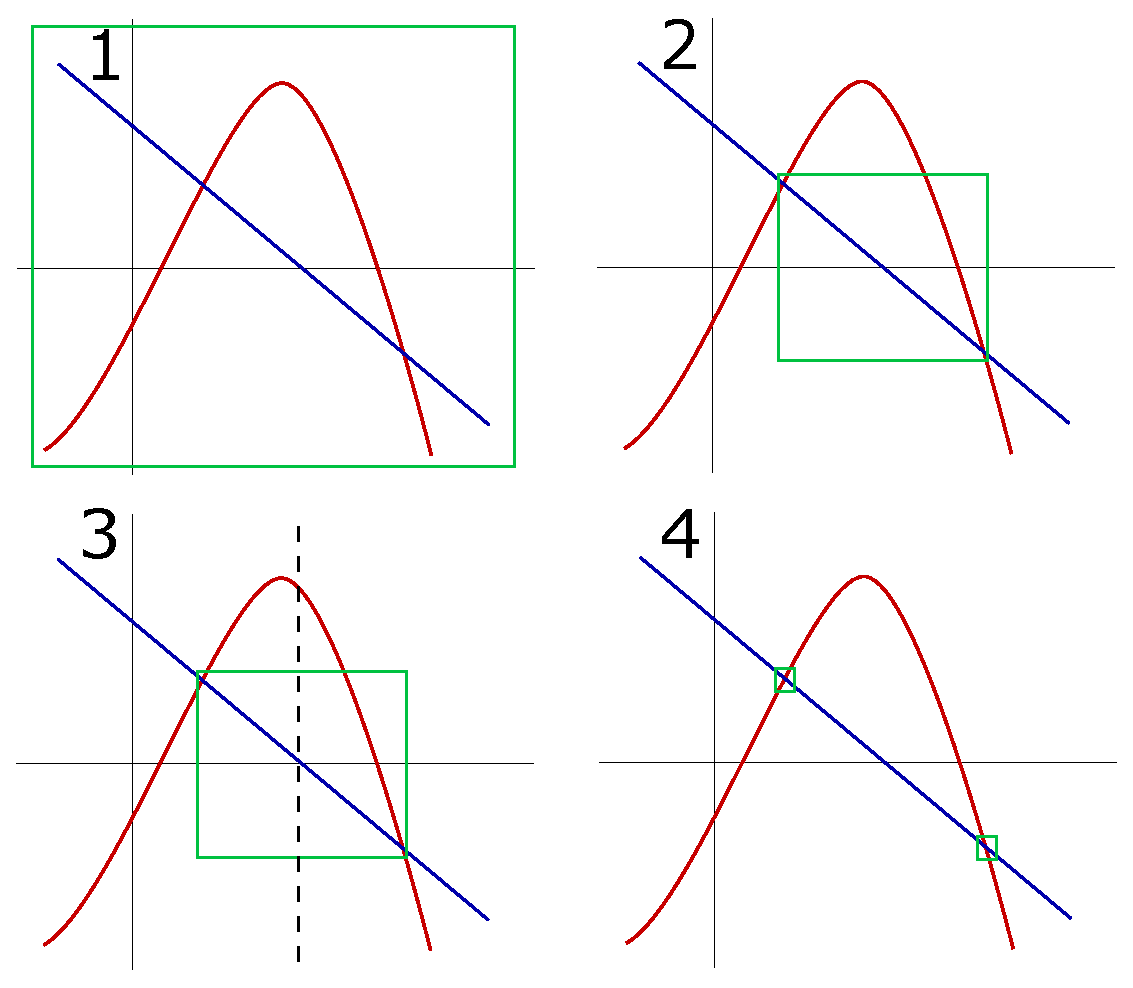
\includegraphics[scale=.7]{img/solving.eps}
\caption{Ukázka průběhu obecného algoritmu Solve s rozdělováním na menší problémy}
\end{figure}



Algoritmům tohoto typu se také říká \emph{branch-and-prune} algoritmy, což je volně přeložitelné jako \uv{větvení a odřezávání větví}. 

Jak bude vidět později, řešič implementovaný v této práci používá podobný algoritmus v rekurzivní variantě (pseudokód konkrétně použité varianty je v patřičné kapitole).

\section{Intervalová aritmetika}
\label{ch:interval_arithmetic}
Intervalová aritmetika je rozšířením aritmetiky reálných čísel na intervaly. (doplnit)

\begin{definition}
\label{def:interval_add}
\emph {Součet intervalů} $a = (x_1; y_1)$ a $b = (x_2; y_2)$ je množina $a + b = \{x+y | x \in a; y \in b \}$, tedy platí, že $(x_1; y_1) + (x_2; y_2) = (x_1 + x_2; y_1 + y_2)$.
\end{definition}

\begin{definition}
\label{def:interval_sub}
\emph {Rozdíl intervalů} $a = (x_1; y_1)$ a $b = (x_2; y_2)$ je množina $a - b = \{x-y | x \in a; y \in b \}$, tedy platí, že $(x_1; y_1) - (x_2; y_2) = (x_1 - y_2; y_1 - x_2)$.
\end{definition}

V případě součinu je situace složitější... 









\section{Vyhledávání, redukce problému a narrowing funkce}
\label{ch:searchReduction}
Rozlišují se dva základní přístupy k řešení CSP a NCSP problémů, a to systematické prohledávání a propagace omezujících podmínek. Základní rozdíl mezi nimi by se dal popsat tak, že zatímco prohledávání hledá platná ohodnocení ve stavovém prostoru, propagace podmínek z něj naopak odstraňuje neplatná ohodnocení. \cite{Vu2005}

Pro řešení problémů s omezujícími podmínkami pomocí prohledávání se mimo jiné dají použít i klasické algoritmy umělé inteligence. Jsou jimi například \emph{hill climbing} (vybere se jedno ohodnocení, vygeneruje se několik sousedů - podobných ohodnocení - a z nich se vybere to nejlepší), či vylepšení tohoto algoritmu, např. \emph{simulated annealing} a \emph{tabu search}. Tyto algoritmy dobře fungují pro klasické CSP problémy s diskrétními doménami proměnných. U NCSP problémů, kde jsou domény proměnných tvořeny intervaly, narážejí na obrovské množství různých ohodnocení (podle požadované přesnosti řešení).



\subsection{Konzistenční techniky}
Konzistenční techniky slouží k odebrání nekonzistentních hodnot z domén proměnných.

\subsection{Algoritmy}
Většina řešičů omezujících podmínek propagací intervalů je založena na snaze dostat omezující podmínky do stavu \emph{hull consistency}, nebo \emph{box consistency} \cite{Benhamou99revisinghull}.

Omezující podmínka je hull konzistentní, pokud se podařilo nalézt nejmenší box, který obaluje všechna řešení splňující danou podmínku. Jsou známy dva základní algoritmy k dosažení hull consistency - \emph{HC3} a \emph{HC4}. Algoritmus HC3 byl navržen jako první z algoritmů pro propagaci intervalů v roce 1997 v článku \cite{Benhamou97applyinginterval}, autoři ho tehdy nazvali jednoduše jako \uv{A narrowing algorithm}. Název HC3 byl vytvořen později v článku \cite{Benhamou99revisinghull}, kde byl uveden i pokročilejší algoritmus HC4.

Tyto algoritmy jsou vhodné především v případě, kdy se jedna proměnná nevyskytuje ve více podmínkách najednou. Pokud tomu tak je, nastává tzv. \emph{dependency problem} (problém závislosti) a HC algoritmy se stávají neefektivními, neboť nalezený obal intervalů může být větší, než je ve skutečnosti potřeba \cite{BenhamouCLPIntervals}.

Oproti tomu jsou BC algoritmy složitější na implementaci než hull consistency algoritmy, efektivně ale řeší situaci, kdy se proměnná objevuje v několika omezujících podmínkách.

Tyto techniky se dají dále kombinovat například s \emph{branch and prune} algoritmy, které umožňují rekurzivně rozpůlit nalezený box a tyto poloviční boxy dále zmenšovat pomocí HC či BC algoritmů. Je tak možné získat několik menších boxů, které budou zahrnovat méně nadbytečných hodnot.











\subsection{Heuristiky}
Heuristiky slouží

\begin{itemize}
  \item Heuristika \emph{dominant-first} se snaží nejprve redukovat domény \uv{dominantních proměnných} - tím jsou myšleny proměnné vyskytující se v původních nerozložených podmínkách,
  \item \emph{small-interval-first/last} se snaží dále zúžit nejužší, resp. nejširší intervaly,
  \item \emph{shrunk-interval-first/last} vybírá nejprve proměnné, jejichž domény byly od běhu nejvíce, resp. nejméně, od začátku běhu algoritmu zmenšeny (vypočítává se kvocient z původní a aktuální velikosti domény),
  \item \emph{max-cand} vybírá proměnnou s nejvyšší levou či pravou mezí domény. Např. proměnná s doménou $(1;6)$ může být vybrána dříve než proměnná s doménou $(1;3)$, protože má vyšší pravou mez.
\end{itemize}



\subsection{Typy heuristik}
Heuristiky používané při řešení problémů s omezujícími podmínkami jsou stále předmětem výzkumu, pro řešení NCSP se dají rozdělit do dvou skupin \cite{feiten10}:

\begin{itemize}
  \item Heuristiky rozhodující podle statických (neměnných) vlastností proměnných, například počtu jejich výskytů, nebo aritmetických operací, kterých se účastní.
  \item Heuristiky rozhodující podle domén proměnných - zúžit širokou doménu může být výhodnější než dále zužovat malou doménu.
\end{itemize}

\begin{itemize}
  \item Statické parametry
    \subitem dominantní vs. nedominantní proměnná
    \subitem vstupní množina podmínek
        \subsubitem počet podmínek, ve kterých se proměnná vyskytuje
        \subsubitem počet dominantních proměnných v constraintu
        \subsubitem operace v constraintu (sčítání/násobení)
  \item Dynamické parametry (tj. mění se během průběhu algoritmu)
    \subitem intervaly
        \subsubitem velikost
        \subsubitem v kladných i záporných hodnotách
    \subitem dvojice se používá ke zredukování domény
\end{itemize}

U dynamických parametrů mám k dispozici celou posloupnost jejich hodnot. V praxi se ale nepoužívá celá posloupnost. Příklady:

\begin{itemize}
  \item poměr aktuální velikosti k původní velikosti
  \item poměr aktuální velikosti k velikosti v minulém průběhu smyčky
  \item číslo průběhu smyčky, kdy se naposledy používala dvojice ke zredukování domény
\end{itemize}


\section{Charakteristiky problémových instancí pro algoritmus HC3}
\begin{itemize}
  \item výskyt jedné proměnné ve více constraintech
  \item počáteční velikosti domén
  \item počet proměnných
  \item počet constraintů
\end{itemize}


\section{Využití v praxi}

\section{Historie NCSP}
 % TODO: Zakomponovat příklad do zbytku práce
Teoretické základy pro problematiku popsanou v bakalářské práci položil John G. Cleary v roce 1987 ve svém článku \emph{Logical Arithmetic}~\cite{cleary87}, kde jsou popsány metody pro redukci domén proměnných v omezujících podmínkách se základními aritmetickými operacemi. Tabulka~\ref{narrowingTable} ukazuje příklad (převzatý z \cite{cleary87}) redukce domény pro omezující podmínku ve tvaru $z = x + y$. Například pro zredukovanou doménu $D_z'$ proměnné $z$ platí $D_z' = D_z \cap (D_x + D_y)$. Aritmetické operace nad intervaly definuje \emph{intervalová aritmetika}. Pro součet uzavřených intervalů platí $\langle a;b \rangle + \langle c;d \rangle = \langle a + c ; b + d \rangle$.

\begin{table}
\centering
\label{narrowingTable}
\begin{tabular}{|l|l|l|l|}
\hline
 Počáteční domény & $x \in \langle 0;2 \rangle$ & $y \in \langle 1;3 \rangle$ & $z \in \langle 4;6 \rangle$  \\ \hline
 $z = x+y$  &  & &  $\langle 1;5 \rangle$  \\ \hline
 $y = z-x$  & & $\langle 2;6 \rangle$  &  \\ \hline
 $x = z-y$  & $\langle 1;5 \rangle$  &  &  \\ \hline
 Nové domény & $x \in \langle 1;2 \rangle$ & $y \in \langle 2;3 \rangle$ & $z \in \langle 4;5 \rangle$ \\ \hline
\end{tabular}
\caption{Příklad redukce domén proměnných v podmínce $z = x + y$}
\end{table}